\subsection{Presentation}
The Voting Classifier is an ensemble model which provides a classification using many other classification models.
In this case, we use all previously trained and tuned models as input to a Voting Classifier

\subsection{Input Models}
\begin{itemize}
    \item K-Nearest-Neighbors: \emph{k = 5}
    \item Decision Tree: \emph{maximum depth = 13}
    \item Support Vector Machine: \emph{gamma = 0.03 ; C = 0.8}
    \item Neural Network (MLP): \emph{alpha = 0.001 ; learning rate (constant) = 0.005}
    \item Stochastic Gradient Descent: \emph{alpha = 0.01}
    \item Random Forest: \emph{max\_depth = 20}
\end{itemize}

\subsubsection{Model Evaluation}
The learning curve shows us the training and validation scores for different data sizes.\\
This way, we are able to say that the score is bounded below 97.5\%, and the model doesn't seem to continue learning after 80000 training rows.
\begin{center}
    \captionsetup{type=figure}
    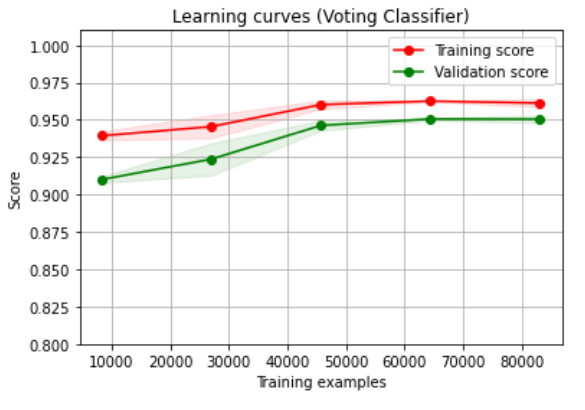
\includegraphics[width=250px]{learning_curve_voting.png}
    \captionof{figure}{Learning Curve for Voting Classifier}
\end{center}
